\subsection{Serial Schedule Generation Scheme} \label{subsec:SGS}

\acp{sgs} stellen für das (M)\ac{rcpsp} wesentliche Techniken zur Erzeugung von Zeitplänen dar. Die am häufigsten in der Literatur verwendeten \acp{sgs} sind \acfp{ssgs} und \acfp{psgs}. Das Prinzip eines \ac{sgs} liegt darin,  vollständige Zeitpläne inkrementell über partielle Zeitpläne aufzubauen. Ein partieller Schedule entspricht einem Zeitplan, welcher unvollständig ist und nicht alle Aktivitäten berücksichtigt, sondern nur eine Teilmenge von Aktivitäten. \cite[vgl.][S. 3 f.]{kolisch_heuristic_1998}\\

Die beiden \ac{sgs} Varianten unterscheiden sich bei der Inkrementierungsweise voneinander. Beim \ac{ssgs} werden $n$ Phasen durchlaufen, wobei in jeder Phase eine Aktivität selektiert wird. Bei dem \ac{psgs} werden bis zu $n$ Phasen durchlaufen. Zu jedem Aktivitätsendzeitpunkt wird überprüft, welche Aktivitäten ausgewählt werden können. Während das \ac{ssgs} aktivitätsinkremental funktioniert, agiert das \ac{psgs} zeitinkremental. \cite[vgl.][S. 3 f.]{kolisch_heuristic_1998}\\

Im Rahmen der Masterthesis wird vermehrt das \ac{mrcpsp} behandelt, welches in Kombination mit dem \acf{psgs} nicht immer eine optimale Lösung darstellt \cite[vgl.][S. 911 f.]{alcaraz_solving_2003} \cite[vgl.][S. 5 f.]{kolisch_heuristic_1998} . Folglich beschränkt sich diese Arbeit auf das \ac{ssgs}. 

\begin{lstlisting}[caption={\ac{ssgs}-Algorithmus (Quelle: \cite[S. 3]{kolisch_heuristic_1998}}), label=lst:sgsalgorithm, mathescape=true, inputencoding={utf8}, extendedchars=false, escapeinside=``]
Init: $F_0$, $S_0 = $ {0},
for g = 1 to n do
    Berechne $\mathcal{D}_g, \mathcal{F}_g, \tilde{\mathcal{R}}_k(t) \, (k \in \mathcal{K}; t \in \mathcal{F}_g)$ 
    W`ä`hle ein $j \in \mathcal{D}$ aus
    $EFT_j$ = $\max_{h \in \mathcal{P}_j} \{ F_h \} + p_j$
    $F_j$ = $\min \{ t \in [EFT_j - p_j, LFT_j - p_j] \cap \mathcal{F}_g | r_{j,k} \leq R_k(\tau), k \in \mathcal{K}, \tau \in [t, t + p_j [\cap \mathcal{F}_g\} + p_j $
    $\mathcal{S}_g$ = $\mathcal{S}_{g - 1} \cup \{ j \}$
$F_{n+1}$ = $\max_{h \in \mathcal{P}_{n+1}} \{ F_h \}$  
\end{lstlisting}

Listing \ref{lst:sgsalgorithm} stellt den \ac{ssgs}-Algorithmus aus dem Manuskript von \cite{kolisch_heuristic_1998} dar. Hierbei wird in jeder Phase $g$ die Mengen $\mathcal{S}_g$ und $\mathcal{D}_g$ berechnet. Die Menge $\mathcal{S}_g$ beinhaltet bereits berücksichtigte Aktivitäten, während $\mathcal{D}_g$ die selektierbaren Aktivitäten für die Phase $g$ beinhaltet. Die Menge $\mathcal{F}_g$ beinhaltet zu $\mathcal{S}_g$ die Endzeiten der einzelnen Aktivitäten. $\tilde{\mathcal{R}}_k(t)$ gibt die Anzahl noch verfügbarer erneuerbarer Ressourcen für die Ressourcenart $k$ zum Zeitpunkt $t$ an. \cite[vgl.][S. 3 f.]{kolisch_heuristic_1998}\\

Abbildung \ref{img:example_ssgs_application} zeigt auf, wie \ac{ssgs} auf einen Projektplan angewendet werden kann, um eine mögliche Lösung für das \ac{rcpsp} zu erhalten. Die Auswahl der Aktivität $j$ aus $\mathcal{D}_g$ erfolgte in dem Beispiel willkürlich. 

\begin{figure}[H]
    \centering
    \noindent\makebox[\textwidth]{%
    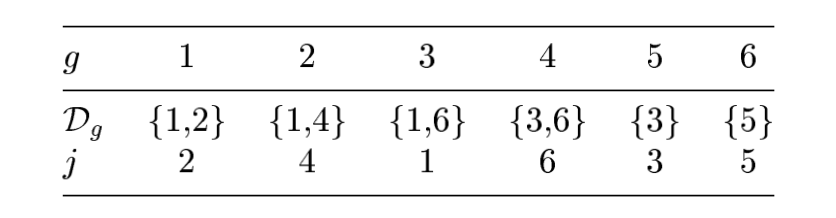
\includegraphics[width=0.6\textwidth]{assets/img/02_Grundlagen/ExampleSSGS.png}
    }
    \caption{\acs{ssgs}-Anwendung auf den RCPSP Beispiel-Projektplan von Abbildung \ref{img:example_rcpsp} zur Erstellung des Zeitplans aus Abbildung \ref{img:example_rcpsp_schedule}}
    \label{img:example_ssgs_application}
    \source{\cite[vgl.][S. 3]{kolisch_heuristic_1998}}
\end{figure}

Aus dem Listing \ref{lst:sgsalgorithm} heraus lassen sich weitere Kennziffern von Aktivitäten innerhalb eines Projektplans erkennen. Im Algorithmus wurden \ac{EFT} und \ac{LFT} verwendet. Diese und \ac{EST} und \ac{LST} sind wesentlich für viele prioritätsbasierte Aktivitätsregeln (vgl. Abschnitt \ref{subsec:SGS_Aktivitaeten}) und für die Robustheitsberechnungen (vgl. Abschnitt \ref{subsec:Praediktive_Methoden}) und werden in der Tabelle \ref{tab:cmr_kennziffern} eingeführt. \\

\begin{table}[H]
\centering
\begin{adjustbox}{width=0.9\columnwidth,center}
\begin{tabular}{|l|l|l|}
\hline
Abk. & Beschreibung \cite[vgl.][S. 126]{burke_project_1999} & Formel \cite[vgl.][S. 127 ff.]{burke_project_1999} \\ \hline
EST  & \begin{tabular}[c]{@{}l@{}}Earliest Starting Time\\ (dt. frühster Startzeitpunkt)\\ stellt den frühstmöglichen Start-\\ zeitpunkt einer Aktivität $j$ dar. \end{tabular}  & $EST_j = \max_{h \in P(j)} \{ EFT(h) \}$ \\ \hline
EFT  & \begin{tabular}[c]{@{}l@{}}Earliest Finishing Time\\ (dt. frühster Endzeitpunkt) \\ stellt den frühstmöglichen End-\\ zeitpunkt einer Aktivität $j$ dar. \end{tabular} & $EFT_j = EST_j + d_j $\\ \hline
LST  & \begin{tabular}[c]{@{}l@{}}Latest Starting Time\\ (dt. spätester Startzeitpunkt)\\ stellt den spätesten Startzeit-\\ punkt einer Aktivität $j$ dar, ohne \\ dass das Projekt in Verzug kommt. \end{tabular} & $LST_j = LFT_j - d_j$ \\ \hline
LFT  & \begin{tabular}[c]{@{}l@{}}Latest Finishing Time\\ (dt. spätester Endzeitpunkt)\\ stellt den spätesten Endzeit-\\ punkt einer Aktivität $j$ dar,\\ ohne dass das Projekt in \\ Verzug kommt. \end{tabular}  & $LFT_j = \min_{h \in P(j)} \{ LST(h) \}$ \\ \hline
\end{tabular}
\end{adjustbox}
\caption{Kennziffern der kritischen Pfadmethode}
\source{In Anlehnung an \cite{burke_project_1999}}
\label{tab:cmr_kennziffern}
\end{table}

\subsubsection{Aktivitäts- und Moduslisten} \label{subsec:SGS_Darstellung}  
Aktivitäts- und Moduslisten sind wesentliche Techniken zur Repräsentation von Lösungen für das (M)\ac{rcpsp}. Insbesondere Metaheuristiken nutzen diese Art der Repräsentation, um aus den Listen Zeitpläne zu transferieren \cite[vgl.][S. 10]{rezaeian_using_2015}, \cite[vgl.][S. 602]{wuliang_improved_2014}, \cite[vgl.][S. 2370]{li_solving_2013}. \\

Zeitpläne im \ac{rcpsp} lassen sich über Aktivitätslisten  $\lambda = \langle j_1, j_2, ..., j_n \rangle$ darstellen. Die Reihenfolge der Aktivitäten entspricht die der Planungsreihenfolge. Folglich müssen die Abhängigkeiten der Aktivitäten zueinander innerhalb der Aktivitätsliste $\lambda$ eingehalten werden. Im Beispiel der Abbildung \ref{img:example_rcpsp_schedule} entspricht die Aktivitätsliste $\lambda = \langle 2, 4, 1, 6, 3, 5 \rangle$. \cite[vgl.][S. 3 f.]{kolisch_heuristic_1998} \\

Für das \ac{mrcpsp} müssen zudem Modi der zugehörigen Aktivitäten berücksichtigt werden. Hierfür werden zusätzlich zu den Aktivitätslisten auch Moduslisten eingesetzt. Eine Modusliste $\mu = \langle m_1, m_2, ..., m_n \rangle$ berücksichtigt ebenfalls die Planungsreihenfolge. Die Länge der Modusliste entspricht der Länge der Aktivitätsliste $|\mu| \equiv |\lambda|$. Folglich können über Aktivitäts- und Moduslisten die Aktivitäten und Modi über die Positionierung zugeordnet werden \cite[vgl.][S. 908]{sebt_efficient_2015}. Für das Beispiel aus Abbildung \ref{img:example_mrcpsp_schedule} entspricht die Aktivitäts- und Modusliste das Tupel $(\lambda, \mu) = (\langle 1, 3, 4, 5, 2, 6, 7 \rangle, \langle 1, 1, 2, 1, 1, 1, 1 \rangle)$. Abbildung \ref{img:ActivityModeListExample} illustriert dieses Beispiel. \\

\begin{figure}[H]
    \centering
    \noindent\makebox[\textwidth]{%
    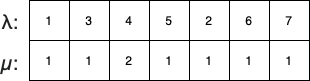
\includegraphics[width=0.45\textwidth]{assets/img/02_Grundlagen/ActivityModeListExample.png}
    }
    \caption{Darstellung der Aktivitäts- und Modusliste $(\lambda, \mu)$ für das MRCPSP Beispiel-Projektplan} 
    \label{img:ActivityModeListExample}
    \source{Eigene Darstellung}
\end{figure}

Eine Lösung für das \ac{mrcpsp} entspricht dem Tupel $I = (\lambda, \mu)$. Für jeden Projektplan existiert mindestens eine optimale Lösung mit der kürzesten Projektdauer $I^* = (\lambda^*, \mu^*)$ \cite[vgl.][S. 4]{kolisch_heuristic_1998}. Das Ziel der (Meta-)Heuristiken liegt darin, die optimale Lösung $I^*$ zu finden oder dieser zumindest sehr nahezukommen. Hierfür müssen Aktivitäts- und Moduslisten ausgewählt, evaluiert und anschließend weitergesucht werden. Abschnitt \ref{subsec:SGS_Aktivitaeten} befasst sich mit Heuristiken zum Finden von Aktivitätslisten, Abschnitt \ref{subsec:SGS_Modi} mit dem Finden von Moduslisten. 

\subsubsection{Prioritätsbasierte Regeln für Aktivitäten} \label{subsec:SGS_Aktivitaeten}

Das \acl{ssgs} stellt eine bedeutende Technik zur Erzeugung von Aktivitätslisten dar. Hierbei wird in jeder Phase $g$ eine Aktivität $j$ aus den möglichen Aktivitäten $\mathcal{D}_g$ ausgewählt. Die Auswahl der Aktivität $j \in \mathcal{D}_g$ gilt es mittels prioritätsbasierten Regeln zu bestimmen. \cite[vgl.][S. 5]{kolisch_heuristic_1998}\\

Prioritätsbasierte Regeln bestehen aus zwei Komponenten, nämlich einer Prioritätswertfunktion $v(j)$ und einem Auswahlparameter $extr$. Die Prioritätswertfunk-tion für Aktivitäten ist über $v: \mathcal{D}_g \rightarrow \mathbb{R}_0$ gemappt und wird über die Prioritätsregeln definiert. Die Funktion gibt für eine mögliche Aktivität $j \in \mathcal{D}_g$ den entsprechenden Prioritätswert gemäß der Regel an. Der Auswahlparameter $extr \in \{ \text{MIN}, \text{MAX} \}$ bestimmt das Extremum. In jeder Phase wird eine Aktivität ausgewählt, die mit dem zugehörigen Prioritätswert dem Extremum aller möglichen Aktivitäten entspricht. Sofern mehrere Aktivitäten dem Extremwert entsprechen, muss eine weitere Heuristik eingeführt werden, wie die Auswahl über die geringste Aktivitätsnummer. \cite[vgl.][S. 6 f.]{schirmer_parameterized_1997}

% Beispiel Auswahl über Prioritätswert

\begin{table}[H]
\centering
\begin{tabular}{r|lll}
Abkürzung & Name & \multicolumn{1}{c}{\begin{tabular}[c]{@{}c@{}}Prioritätsregel-\\funktion $v(j)$\end{tabular}} & \multicolumn{1}{c}{\begin{tabular}[c]{@{}c@{}}Auswahl-\\parameter $extr$\end{tabular}} \\ \hline
GRPW & Greatest Rank Positional Weight & $d_j + \sum_{i \in S(j)} d_i $ & MAX \\
LFT & Latest Finish Time & $LFT_j $ & MIN \\
LST & Latest Start Time & $LST_j $ & MIN \\
MSLK & Minimum Slack & $LFT_j - EFT_j$ & MIN \\
MTS & Most Total Successors & $|S(j)| $ & MAX \\
\end{tabular}
\caption{Prioritätsregeln für Aktivitäten}
\label{tab:ActivityRules}
\source{\cite[vgl.][S. 6]{kolisch_heuristic_1998}}
\end{table}

Die in Tabelle \ref{tab:ActivityRules} aufgeführten etabilierten Regeln werden genutzt, um anhand der Prioritätsregelfunktion $v(j)$ gemäß Auswahlparameter $extr$ die zugehörige Aktivität $j$ auszuwählen. Tabelle \ref{tab:ActivityRulesExample} zeigt ein Beispiel bei Anwendung einer beliebigen Prioritätsregelfunktion $v(j)$ auf. Sofern der Auswahlparameter $extr = \text{MAX}$ entspricht, wird in der Phase $g$ die Aktivität 3 ausgewählt, bei $extr = \text{MIN}$ die Aktivität 2.  
 
\begin{table}[H]
\centering
\begin{tabular}{r|c|c|c|c}
$j \in \mathcal{D}_g$ & 1 & 2 & 3  & 4 \\ \hline
$v(j)$ & 5 & 3 & 12 & 4
\end{tabular}
\caption{Beispiele von Prioritätswerten von den möglichen Aktivitäten $j \in \mathcal{D}_g$ einer Phase $g$}
\label{tab:ActivityRulesExample}
\source{Eigene Darstellung}
\end{table}


\subsubsection{Selektionsregeln für Modi} \label{subsec:SGS_Modi}
Um beim \ac{mrcpsp} Zeitpläne zu erzeugen, müssen neben den Aktivitätslisten auch Moduslisten generiert werden. Des Weiteren besteht beim \ac{mrcpsp} die Problematik, dass bei Anwendung der Prioritätsregeln für eine Aktivität mehrere Modi mit unterschiedlichen Ressourcen- und Zeitanforderungen zur Verfügung stehen. Folglich werden Selektionsregeln für Modi benötigt, welche analog zu den Prioritätsregeln für Aktivitäten funktionieren. \\


\begin{table}[H]
\centering
\resizebox{\textwidth}{!}{%
\begin{tabular}{r|lll}
Abkürzung & Name & \multicolumn{1}{c}{\begin{tabular}[c]{@{}c@{}}Selektionsregel-\\funktion $s(j, m)$\end{tabular}} & \multicolumn{1}{c}{\begin{tabular}[c]{@{}c@{}}Auswahl-\\parameter $extr$\end{tabular}} \\ \hline
LPSRD & Least Product Sum of Res. and Dur. & $\sum_{l=1}^{|L|} (c_{j,m,l} \cdot d_{j,m})$ & MIN \\
LRP & Least Resource Proportion & $\max (\frac{r_{j,m,k}}{|K|})$ & MIN \\
LRS & Least Sum of Non-renewable Resource & $\sum_{l=1}^{|L|}  \frac{c_{j,m,l}}{R^v_k}$ & MIN \\
LTRU & Least Total Resource Usage & $\sum_{l=1}^{|L|} c_{j,m,l}$ & MIN \\
SFM & Shortest Feasible Mode & $d_{j,m}$ & MIN \\

\end{tabular}
}%
\caption{Selektionsregeln für Modi}
\label{tab:ModeRules}
\source{\cite[vgl.][S. 5046]{chen_entropy-based_2014}}
\end{table}

Die in Tabelle \ref{tab:ModeRules} aufgeführten etabilierten Regeln werden genutzt, um anhand der Selektionsregelfunktion $s(j, m)$ gemäß Auswahlparameter $extr$ den zugehörigen Modus $m \in M_j$ einer Aktivität $j$ auszuwählen. Tabelle $\ref{tab:ModesRulesExample}$ zeigt ein Beispiel bei Anwendung einer beliebigen Prioritätsregelfunktion $v(j)$ und Selektionsregelfunktion $s(j, m)$ auf. Um die Aktivitätsregelfunktion anwenden zu können, müssen vorher die Modi selektiert werden \cite[vgl.][S. 5046]{chen_entropy-based_2014}. Die Selektion der Modi und Aktivitäten geschieht im Beispiel über $extr = \text{MAX}$. Für alle möglichen Aktivitäten der Phase $j \in \mathcal{D}_g$ wird somit der erste Modus ausgewählt. Im Anschluss können die Aktivitäten über die Prioritätsregeln ausgewählt werden (vgl. Abschnitt \ref{subsec:SGS_Aktivitaeten}). 


\begin{table}[H]
\centering

\begin{tabular}{r|cc|cc|cc|cc}
$j \in \mathcal{D}_g$  & \multicolumn{2}{c|}{1} & \multicolumn{2}{c|}{2} & \multicolumn{2}{c|}{3} & \multicolumn{2}{c}{4} \\ \hline
$m \in M_j$ & \multicolumn{1}{c|}{1} & 2 & \multicolumn{1}{c|}{1} & 2 & \multicolumn{1}{c|}{1} & 2 & \multicolumn{1}{c|}{1} & 2 \\ \hline
$s(j, m)$                 & \multicolumn{1}{c|}{5} & 3 & \multicolumn{1}{c|}{2} & 1 & \multicolumn{1}{c|}{5} & 4 & \multicolumn{1}{c|}{7} & 7 \\ \hline
$v(j)$                      & \multicolumn{2}{c|}{5} & \multicolumn{2}{c|}{3} & \multicolumn{2}{c|}{12} & \multicolumn{2}{c}{2} 
\end{tabular}%

\caption{Beispiele von Prioritäts- und Selektionswerten von den möglichen Aktivitäten $j \in \mathcal{D}_g$ und Modis der Aktivitäten einer Phase $g$}
\label{tab:ModesRulesExample}
\source{Eigene Darstellung}
\end{table}

\subsubsection{Sampling als Multi Pass Methode} \label{subsec:SGS_RBBRS}

Das Anwenden der Aktivitäts- und Modusregeln führt innerhalb eines \ac{ssgs} zu einem einzigen Zeitplan und wird somit als eine Single Pass Methode klassifiziert \cite[vgl.][S. 6]{kolisch_heuristic_1998}. Das Anwenden dieser Heuristiken führt bei gleichbleibendem Input zudem immer zu identischen Ergebnissen und sind folglich deterministisch \cite[vgl.][S. 4]{schirmer_parameterized_1997}. Dennoch besteht das Interesse eine breitere Menge an möglichen Zeitplänen zu untersuchen, um durchaus bessere Ergebnisse als das direkte Anwenden der Regeln zu erhalten.\\

Unter Multi Pass Methoden werden wiederum Verfahren bezeichnet, die in der Lage sind, mehrere Zeitpläne zu generieren. Hierunter fallen Verfahren, wie das Anwenden von mehreren Regeln, aber auch das Sampling. Für jede mögliche Aktivität einer Phase $j \in \mathcal{D}_g$ und deren jeweiligen Modi $m \in M_j$ ist hierbei ein Wahrscheinlichkeitswert gemäß Funktion $p(x) \in [0, 1]$ vorgesehen, welche für die Entscheidungsmenge aufkommuliert stets 1 ergeben muss. Aus der Entscheidungsmenge wird im Anschluss gemäß der Wahrscheinlichkeit die Aktivität bzw. der Modus ausgewählt. Die Wahrscheinlichkeitsfunktion $p(x)$ wird anhand von Sampling Methoden definiert. \cite[vgl.][S. 7 f.]{kolisch_heuristic_1998} Aufgrund der Einfachheit beziehen sich die Formeln der folgenden vorgestellten Sampling Methoden nur auf die Aktivitätsauswahl. Diese lassen sich jedoch ohne weiteres auch auf die Modusauswahl ableiten. \\

Die einfachste Sampling Methode ist \ac{RS}. Hierbei ist die Wahrscheinlichkeit $p(x)$ innerhalb der Entscheidungsmenge gleichverteilt $p(j) = \dfrac{1}{|\mathcal{D}_g|}$. \cite[vgl.][S. 7]{kolisch_heuristic_1998} Hierbei werden Prioritäts- und Selektionregeln ignoriert und gänzlich zufällige Zeitpläne erzielt. \\

Eine weitere Sampling Methode ist \ac{BRS}. Die Wahrscheinlichkeit $p(x)$ hängt hierbei direkt von der Prioritäts- und Selektionsregel ab $p(j) = \dfrac{v(j)}{\sum_{i \in \mathcal{D}_g} v(i)}$. \cite[vgl.][S. 7]{kolisch_heuristic_1998} \\

Über \ac{RBRS} ist es zudem möglich, die Wahrscheinlichkeit $p(x)$ über einen Regretwert (dt. Reuewert) zu beeinflussen \cite[vgl.][S. 12]{schirmer_parameterized_1997}. Dies führt dazu, dass die Aktivitäts- und Moduslisten gemäß der Prioritäts- und Selektionsregeln mehr oder weniger variieren können. Die Wahrscheinlichkeit $p(x)$ lässt sich über die folgenden Funktionen gemäß \cite[vgl.][S. 12]{schirmer_parameterized_1997} definieren: 
\begin{align}
    v'(j) &= 
    \left\{\begin{array}{ll} 
        \max_{i \in \mathcal{D}_n}(v(i)) - v(j) & \text{wenn extr = min} \\
        v(j) - \min_{i \in \mathcal{D}_n}(v(i)) & \text{wenn extr = max} \\
     \end{array}\right.  \\
    v''(j) &= (v'(j) + \epsilon)^\alpha  \\
    p(j) &= \frac{v''(j)}{\sum_{i \in D_n} v''(i)}
\end{align}

$v'(j)$ und $v''(j)$ stellen die Regrets dar. Beim \ac{RBRS} werden die Regrets zudem mit $\epsilon = \mathbb{R}_{>0}$ und $\alpha = \mathbb{R}_{\geq0}$ parametrisiert. $\epsilon$ garantiert, dass $v''(j) \neq 0$. Dies ist relevant, um innerhalb der Wahrscheinlichkeitsfunktion $p(x)$ Divisionen durch 0 zu vermeiden. $\alpha$ regelt den Einfluss der Prioritäts- und Selektionsregelfunktion auf den Wahrscheinlichkeitswert. Bei einem hohen Wert verstärkt sich der Einfluss, bei einem niedrigen Wert verringert sich dieser. Bei $\alpha = 0$ ist die Prioritäts- und Selektionsregelfunktion irrelevant und folglich sind die Wahrscheinlichkeiten innerhalb der Entscheidungsmenge gleichverteilt, identisch zum \ac{RS}. Bei $\alpha = \infty$ sind die Wahrscheinlichkeiten so angeordnet, dass die Aktivität oder der Modus deterministisch ausgewählt werden kann, identisch zur Single Pass Methode. \cite[vgl.][S. 12 f.]{schirmer_parameterized_1997} \\

Die Funktionsweise der vorgestellten Multi Pass Samplingverfahren lassen sich in Tabelle \ref{tab:ExampleSampling} aufbauend auf dem Beispiel aus Abschnitt \ref{subsec:SGS_Aktivitaeten} verdeutlichen. Für dieses Beispiel liegt der Extremwert für die zu betrachtende Prioritätsregel bei $extr = \text{MAX}$. Sofern \ac{RBRS} als Sampling-Methode ausgewählt wurde, so wird z. B. die Aktivität 3 mit einer 80 prozentigen Wahrscheinlichkeit selektiert. Wenn $\alpha = \infty$, dann wird das Ergebnis gemäß der regelbasierten Single Pass Methode deterministisch ausgewählt.  




\begin{table}[H]
\centering
\begin{tabular}{r|l|l|l|l}
$j \in \mathcal{D}_g$                      & \multicolumn{1}{c|}{1} & \multicolumn{1}{c|}{2} & \multicolumn{1}{c|}{3}  & \multicolumn{1}{c}{4} \\ \hline
$v(j)$                                     & \multicolumn{1}{c|}{5} & \multicolumn{1}{c|}{3} & \multicolumn{1}{c|}{12} & \multicolumn{1}{c}{4} \\ \Xhline{2\arrayrulewidth}
\acf{RS} & 0.25                   & 0.25                   & 0.25                    & 0.25                  \\ \hline
\acf{BRS}& 0,21                   & 0,13                   & 0,50                    & 0,16                  \\ \hline
\acf{RBRS} & 0,10                   & 0,03                   & 0,80                    & 0,07                  \\ \hline
\ac{RBRS} mit $\alpha = 0$                      & 0.25                   & 0.25                   & 0.25                    & 0.25                  \\ \hline
\ac{RBRS} mit $\alpha = \infty$                      & 0.00                   & 0.00                   & 1.00                    & 0.00                 
\end{tabular}
\caption{Selektionswahrscheinlichkeiten $p(j)$ für die vorgestellten Sampling-Verfahren mit $|\mathcal{D}_g| = 4$ und $extr = \text{MAX}$ }
\label{tab:ExampleSampling}
\source{In Anlehnung an \cite[vgl.][S. 8]{kolisch_heuristic_1998}}
\end{table}
